\documentclass[main]{subfiles}

\begin{document}

\chapter{Hardware}
La elecci\'on del Hardware significa una parte muy importante del Proyecto, ya que las decisiones tomadas condicionan el resto del mismo. Una mala elecci\'on de alguno de los componentes puede resultar en complicaciones no previstas a la hora de la ejecuci\'on, causando contratiempos inesperados y trabajo excesivo. Es necesario, entonces, el estudio detallado de cada uno de los componentes a utilizar, comparando caracter\'isticas, rendimientos y utilidades.\\

Elegir adecuadamente el Hardware necesario agiliza las etapas siguientes de todo el Proyecto. Resulta fundamental la toma de buenas decisiones, las cuales deben estar basadas en un previo estudio de cada etapa del proyecto, sus requerimientos, un estudio comparativo de las posibles soluciones y el conocimiento cabal de los componentes a utilizar.\\

\section{Plataforma f\'isica: Cuadric\'opteros}


A la hora de la planificaci\'on del Proyecto se plantean dos opciones que se diferencian b\'asicamente en el punto de partida. Ambas tienen como objetivo principal dise\~nar e integrar un sistema de control que permita al cuadric\'optero mantener un vuelo aut\'onomo, pero una de ellas consta adem\'as del dise\~no y el armado del mismo. \\Esta \'ultima incluye desaf\'ios de ingenier\'ia mec\'anica, conocimientos de resistencia, flexibilidad y peso de materiales, as\'i como tambi\'en diversas complicaciones a la hora de fabricar y armar las partes. \\

Teniendo en cuenta que se trata de un proyecto con tiempo acotado y su objetivo se centra en el control del veh\'iculo, la necesidad de partir de hardware ya construido resulta imperiosa. La plataforma escogida es el cuadric\'optero Turbo Ace X720, este mismo cuadric\'optero es conocido adem\'as como LotusRc 850.\\

Esta plataforma es controlada por un usuario a trav\'es de un control remoto. El sistema receptor ( ) - CPU se encarga de setear la velocidad angular de cada motor en funci\'on de la se\~nal recibida. 
%TODO nombre del control y receptor
 
\subsubsection*{Motores}
Los motores de la plataforma son \emph{Brushless}, estos son motores el\'ectricos alimentados con corriente continua. Tienen un sistema de conmutaci\'on el\'ectrico y presentan relaciones lineales entre \emph{Corriente} y \emph{Torque} y entre \emph{Frecuencia} y \emph{velocidad}. Son com\'unmente utilizados en veh\'iculos radio-controlados por su gran eficiencia, potencia, durabilidad y su bajo peso en comparaci\'on con los tradicionales motores \emph{Brushed}. Sin embargo, los motores de CC \emph{Brushless} son mucho m\'as complicados de controlar, ya que la fase var\'ia con la rotaci\'on del motor. Para controlarlos debe utilizarse un dispositivo llamado \emph{Controlador el\'ectrico de velocidad}, o \textbf{ESCs}. Com\'unmente los ESCs se clasifican seg\'un su corriente m\'axima, por ejemplo 10 amp\'eres o 10A.\\

El comando de los motores se basa en el protocolo $I^2C$ funcionando a una frecuencia de $400kHz$.  

\subsubsection*{Peso}

	La carga \'util que el dispositivo pueda soportar juega un papel fundamental. Vale recordar que, adem\'as de toda la instrumentaci\'on que incluye el cuadric\'optero, se incorporar\'a un microprocesador, una bater\'ia independiente para su alimentaci\'on, un gir\'oscopo, un aceler\'ometro, un GPS y alguna interfaz para la comunicaci\'on. A su vez es interesante conservar la posibilidad de integrar una c\'amara fotogr\'afica convencional ya que puede ser de gran utilidad para numerosas aplicaciones. La fuerza que los motores pueden realizar es acotada, por lo que el peso del dispositivo influye directamente en la carga \'util del mismo. Para esta plataforma la carga adicional que puede agregarse es de 1300g incluyendo bater\'ia. 

\subsubsection*{Tiempo de vuelo}

El tiempo de vuelo puede resultar cr\'itico seg\'un la aplicaci\'on considerada, en este caso no ser\'a posible superar los 20 minutos de vuelo utilizando una bater\'ia de LiPo de 5300mAh. 

\subsubsection*{Instrumentaci\'on}

	La instrumentaci\'on que el dispositivo brinda est\'a destinada al manejo mediante el control remoto. La misma incluye un aceler\'ometro y un gir\'oscopo de 3 ejes, un bar\'ometro y poseen alg\'un sistema de estabilizaci\'on incluido, de forma de facilitar el control. \\

Lamentablemente el software presente en la CPU es privativo por lo tanto reutilizarlo parece una tarea muy dificultosa, del mismo modo obtener la lectura de los sensores presentes tampoco parece una tarea sencilla. Por dicho motivo se opta por dotar al sistema de instrumentaci\'on adicional. 

En la figura \ref{fig:cuadricoptero} se puede apreciar una imagen de la plataforma utilizada.
\begin{figure}[H]
	\centering
	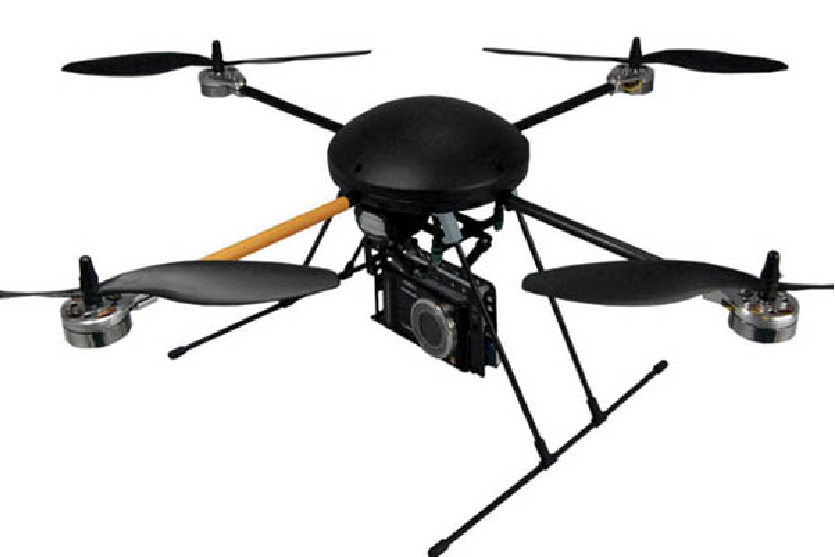
\includegraphics[width=0.5\textwidth]{./pics_eleccion_hardware/turboace.png}
	\caption{Turbo Ace X720}
	\label{fig:cuadricoptero}
\end{figure}


\section{Inteligencia}

Adem\'as de la plataforma f\'isica, deben seleccionarse componentes electr\'onicos capaces de procesar la informaci\'on proveniente de los sensores, computar y ejecutar los algoritmos de control y generar las se\~nales necesarias para transmitir las instrucciones a los motores.\\

La soluci\'on implementada se basa en la plataforma de desarrollo \emph{Beagleboard}. Esta plataforma posee un microprosesador TI ARM Cortex A8 de 1GHz y un DSP TMS320C64x+ de 800MHz, la memor\'ia RAM de la misma es de 512 Mb y si bien no tiene memoria no volatil soporta tarjetas SD de hasta 4GB.


\subsection*{Dimensiones y peso}

Si bien no resulta una caracetr\'istica determinante, es conveniente que las dimensiones y peso de la placa elegida sean lo menores posibles, de forma de no ocupar gran parte de la carga \'util del cuadric\'optero con electr\'onica asociada a la inteligencia implementada. El peso de la Beagleboard y una bater\'ia asociada diseñada especialmente para esta plataforma es de 76 gramos y sus dimensiones son $10cm\times8.5cm\times2cm$. La autonom\'ia de la bater\'ia es de aproximadamente 2 horas. \\

\subsection*{Programaci\'on y Sistema Operativo}

Es importante tener en cuenta como ser\'a realizada la programaci\'on de los sistemas considerados (d\'onde se almacena el programa, hardware necesario para la programaci\'on, etc.) En particular, es conveniente poder contar con alg\'un sistema operativo que facilite la tareas de programaci\'on, testeo y debugging.\\

La BeagleBoard ofrece la posilibidad de cargar un kernel de \emph{Linux} desde una tarjeta SD. Esto ofrece una amplia gama de posibilidades. A modo de ejemplo podemos nombrar las facilidades que implica en cuanto a la comunicaci\'on. La plataforma dispone de una interfaz ethernet y cuatro puertos USB. Al disponer de un sistema operativo, los \emph{drivers} de dichas interfaces se pueden utilizar obteniendo as\'i la posibilidad de realizar ajustes sobre el sistema a trav\'es de la interfaz ethernet o de una interfaz WiFi agregando el m\'odulo USB (Belkin wireless G). Adem\'as se dispone de un puerto serie. 

\subsection*{Puertos e I/Os}

Las posibilidades que ofrece la Beagleboard en cuanto a puertos de entrada y salida son muy considerables. A modo de ejemplo se tienen cuatro puertos USB, una interfaz ethernet un puerto de expansi\'on de 28 pines de proposito general y un puerto serie. En lo que respecta a la soluci\'on implementada es importante destacar que los pines 23 y 24 pueden ser programados para comunicarse a trav\'es del protocolo $I^2C$ fundamental para enviar comandos a los motores. Los pines 23 y 24 corresponden a las lineas de datos y al reloj respectivamente. Por otra parte, los pines 8 y 6 pueden ser configurados para funcionar como pines de transmici\'on y recepci\'on de un puerto serie. Esto ser\'a fundamental para la comunicaci\'on con algunos de los sensores.\\

\section{Instrumentaci\'on}
\vspace*{15pt}
Para poder controlar el sistema es importante poder conocer los valores que toman las variables del mismo. Como se ver\'a en el cap\'itulo sobre el desarrollo del modelo f\'isico del cuadric\'optero, las variables que es necesario conocer son:

\begin{itemize}
\item La orientaci\'on del sistema en el sistema de coordenadas utilizado
\item La altura del sistema en el sistema de coordenadas utilizado
\item La aceleraci\'on en las tres coordenadas
\item La velocidad angular del sistema seg\'un tres ejes de rotaci\'on
\end{itemize}

Por dicho motivo parece imprescindible dotar al sistema de sensores capaces de medir dichas magnitudes.
\subsection{IMU}

\subsubsection{Aceler\'ometro}
\label{acelerometro}

Un aceler\'ometro es un dispositivo capaz de medir su aceleraci\'on propia en el marco de referencia de la ca\'ida libre. Esto implica que el dispositivo no mide siempre su cambio de velocidad en el espacio.\\
Por ejemplo, la medida de un aceler\'ometro en ca\'ida libre ser\'a cero a pesar de que su velocidad crezca, de la misma forma se puede observar que un aceler\'ometro en reposo respecto de la Tierra, no dar\'a una medida nula, sino que por el contrario medir\'a como aceleraci\'on g.\\

Existen diversos tipos de aceler\'ometro, en este caso se eligi\'o trabajar con un aceler\'ometro contenido en un circuito integrado (tecnolog\'ia MEMS). Las razones de esta elecci\'on son fundamentalmente tama\~no y peso (cr\'iticos en la aplicaci\'on) y econ\'omicos. Los mismos son m\'as peque\~nos, livianos y baratos que otras tecnolog\'ias.\\
Dicho aceler\'ometro procesa las medidas y las convierte a una salida el\'ectrica; la forma de dicha salida depende si el integrado es anal\'ogico o digital.\\
Los aceler\'ometros basados en tecnolog\'ias MEMS miden cambios internos de la transferencia de calor causada por la aceleraci\'on, ofreciendo ventajas significativas sobre el empleo de una estructura tradicional s\'olida de masas de prueba.\\
Ya que la masa de prueba en el dise\~no de los sensores MEMS son mol\'eculas de gas, las estructuras m\'oviles mec\'anicas son eliminadas dentro del aceler\'ometro.\\

%TODO Referencia a MEMS
Un aceler\'ometro de tres ejes no es otra cosa que un aceler\'ometro capaz de medir su aceleraci\'on propia en tres ejes de coordenadas.\\


El aceler\'ometro cumple dos roles fundamentales. El primero es que, bajo el supuesto que las aceleraciones a las cuales se ver\'a sometido el sistema no son comparables con $g$ el mismo sirve para determinar con gran precisi\'on los \'angulos de Pitch y de Roll. El segundo, es que nos permite obtener una estimaci\'on de la velocidad al integrar su medida.  
 
\subsubsection{Gir\'oscopo}
\label{giro}

Un gir\'oscopo es un instrumento que mide la velocidad angular del sistema en un sistema de referencia solidario a si mismo. Las mismas restricciones sobre tama\~no, peso y costos que se aplicaban para el aceler\'ometro se aplican aqu\'i. Por dicho motivo se vuelve a optar por un instrumento de tecnolog\'ia MEMS.\\ 

Desde el punto de vista te\'orico, procesando la informaci\'on obtenida a partir del aceler\'ometro y del gir\'oscopo se puede conocer en todo momento la posici\'on del sistema y su orientaci\'on a partir de las condiciones iniciales.\\

En la pr\'actica, sin embargo, esto no sucede as\'i. Todas las medidas realizadas tienen un cierto error. Para obtener la orientaci\'on y la posici\'on a cada instante se deben integrar las medidas obtenidas, por lo tanto, se integra tambi\'en el error cometido. Esto produce una acumulaci\'on de errores que afecta de forma considerable el resultado final luego de cierta cantidad de muestras.\\
Parece razonable, entonces, poder cotejar los datos que se obtienen mediante este m\'etodo con datos obtenidos mediante otras fuentes. Es a partir de esta problem\'atica que surge la necesidad de contar con un GPS. Se puede, cada cierto intervalo de tiempo, observar en cuanto difieren los resultados obtenidos integrando las medidas de los sensores con los datos que aporta el GPS, logrando de esta forma corregir los errores debido al \emph{integration drift}.

\subsubsection{Sensor de presi\'on}

Si bien un dispositivo GPS provee una estimaci\'on de la altura a la que se encuentra, la misma resulta ser poco exacta y confiable, por depender fuertemente de la cantidad de sat\'elites vistos por el GPS as\'i como por el efecto del rebote de las ondas en estructuras cercanas (resulta particularmente cr\'itico el efecto de los rebotes en el piso, los cuales dan poca precisi\'on a la medida de altura al estar muy cerca del suelo). Por este motivo es necesario contar con un sensor de presi\'on absoluta que nos permita determinar la altura del cuadric\'optero en forma independiente al resto de los sensores. La medida de presi\'on debe ser absoluta pues es este tipo de medidas las que pueden ser traducidas a altura en forma r\'apida y confiable.

\subsubsection{Magnet\'ometro}

Si bien el sistema contar\'a con gir\'oscopos que permitir\'an, a trav\'es de integraci\'on, estimar la orientaci\'on del cuadric\'optero, dicha estimaci\'on est\'a sujeta a los errores asociados a este tipo de sensores (errores de drift e integraci\'on, entre otros), siendo adem\'as dicha medida una medida diferencial, teniendo como \'unica referencia la orientaci\'on inicial del cuadric\'optero. Eso por ello que resulta conveniente contar con un magnet\'ometro que permita tener una medida absoulta y confiable del \'angulo de Yaw, la cual puede ser entonces complementada y corregida mediante la informaci\'on obtenida mediante la integraci\'on de la informaci\'on generada por el gir\'oscopo.

\subsubsection{Sensor de temperatura}

Si bien el control del sistema no depende directamente de la temperatura, los instrumentos a utilizarse est\'an construidos con cierta tecnolog\'ia que presenta dependencia con (y por ende tendr\'a errores asociados a) la temperatura. El contar con un sensor de temperatura permitir\'a sensar la misma y realizar correcciones en tiempo real que permitan minimizar dicho errores.\\

La Mongoose 9DoF IMU posee todos los sensores que se han nombrado hasta aqu\'i excepto el GPS. La misma posee adem\'as un micropresador con facilidades para ser programado, puediendo as\'i realizar un preprocesamiento de los datos antes de realizar la estimaci\'on del estado. Entre las modificaciones realizadas las m\'as importantes son un aumento y una estabilizaci\'on de la frecuencia de muestreo y la conversi\'on de los datos de salida de formato ASCII a binario. Esto \'ultimo permite una mayor velocidad de transmisi\'on de los mismos a trav\'es del puerto serie de la Mongoose. En la figura \ref{fig:mongoose} se puede observar dicha placa de instrumentaci\'on. Las caracter\'isticas de dicha placa pueden consultarse en \ref{chap:anexo_mongoose}.


\begin{figure} 
  \centering
  \subfloat[Mongoose]{\label{fig:mongoose}
  		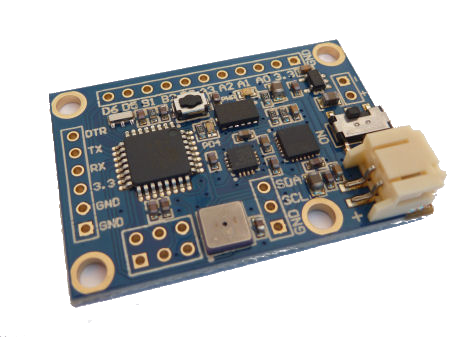
\includegraphics[width=0.3\textwidth]
  			{./pics_eleccion_hardware/Mongoose.png}}
  \subfloat[Canmore GT-730F]{\label{fig:gps} 
  		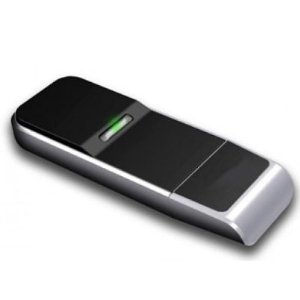
\includegraphics[width=0.3\textwidth]
  			{./pics_eleccion_hardware/gps.jpg}}
  
  \caption{Instrumentaci\'on}
  \label{fig:intrumentacion}
\end{figure}




\subsection{GPS}

La elecci\'on del GPS se bas\'o cas\'i totalmente en lograr la simplicidad del sistema. Exist\'ian muchas opciones, placas de diversos tama\~nos, con diversos tama\~nos de antenas, pero todas con similares especificaciones.\\

Las placas candidatas a estar a cargo de la inteligencia contaban con interfaces USB, por lo que se opt\'o por comprar un dongle GPS, cuyas especificaciones son similares a las del resto de las opciones, y se puede comunicar via USB. Existen drivers para dicho GPS en linux, por lo que la comunicaci\'on con el mismo no deber\'ia ser un problema.\\
\\
Se opt\'o por utilizar un GPS \textit{Canmore GT-730F}.

\end{document}

%Algunos layouts para poner im\'agnenes. Copien y peguen nom\'as. Hay figura com\'un, dos figuras en 1 onda fig 3a y 3b, wrapfigures y una matriz de figuras. Ta bueno, todas quedan lindas y andan bien.
%
%\begin{figure}[h!]
%	\centering
%	\includegraphics[width=0.75\textwidth]{./pics_eleccion_hardware/		.eps}
%	\caption{		}
%	\label{fig:		}
%\end{figure}
%
%\begin{figure} [h!]
%  \centering
%  \subfloat[caption 1]{\label{fig:		}
%  		\includegraphics[width=0.45\textwidth]
%  			{./pics_eleccion_hardware/		.eps}}
%  \subfloat[caption 2]{\label{fig:		} 
%  		\includegraphics[width=0.45\textwidth]
%  			{./pics_eleccion_hardware/ 		.eps}}
%  \caption{Caption general}
%  \label{fig:	label general	}
%\end{figure}
%
%\begin{wrapfigure}{l}{0.6\textwidth}
%  \vspace{-20pt}
%  \begin{center}
%    \includegraphics[width=0.45\textwidth]
%    	{./pics_eleccion_hardware/		.eps}
%  \end{center}
%  \vspace{-20pt}
%  \caption{		}
%  \label{ 		}
%  \vspace{-10pt}
%\end{wrapfigure}
%
%\begin{figure} [h!]
%  \begin{center}
%    \begin{tabular}{cc}
%      \resizebox{50mm}{!}
%      	{\includegraphics{./pics_eleccion_hardware/ 	.eps}} &
%      \resizebox{50mm}{!}
%      	{\includegraphics{./pics_eleccion_hardware/	.eps}} \\
%      \resizebox{50mm}{!}
%      	{\includegraphics{./pics_eleccion_hardware/	.eps}} &
%      \resizebox{50mm}{!}
%      	{\includegraphics{./pics_eleccion_hardware/	.eps}} \\
%    \end{tabular}
%    \caption{ 		}
%    \label{ 		}
%  \end{center}
%\end{figure}